\documentclass{ieee-ojvt}
\usepackage{cite}
\usepackage{amsmath,amssymb,amsfonts}
\usepackage{algorithmic}
\usepackage{graphicx,color}
\usepackage{textcomp}
\def\BibTeX{{\rm B\kern-.05em{\sc i\kern-.025em b}\kern-.08em
    T\kern-.1667em\lower.7ex\hbox{E}\kern-.125emX}}
\AtBeginDocument{\definecolor{ojcolor}{cmyk}{0.93,0.59,0.15,0.02}}
\def\OJlogo{\vspace{-12pt}
\includegraphics[height=24pt]{ojvt-logo.png}}

% Figures: Fig. 1 is the unmodified notebook PNG; Figs. 2 and 3 are the presentation-only
% re-exports of paper_taes/figures (replot_paper_figures.py, data in fig_data.npz).
\graphicspath{{figures/}}

% DOIs are stored in the `note' field of References.bib as \href{url}{doi}; the class has
% no hyperref, so typeset the DOI text with breakable \url line breaking.
\usepackage{url}
\providecommand{\href}[2]{\url{#2}}

% --- measured quantities (Section U of the companion notebook); single source of truth ---
\newcommand{\PLNCH}{11\,700}          % active channels per context
\newcommand{\PLMASEL}{$77$~ms}        % MaxActive threshold sweep, decision only
\newcommand{\PLMASTEP}{$95$~ms}       % MaxActive full link update, fixed beam (11 contexts)
\newcommand{\PLMASTEPBW}{$91$~ms}     % + beamwidth search (the 3 comparable contexts)
\newcommand{\PLPREDUS}{$0.9$~ms}      % surrogate: feature extraction + inference

\begin{document}
\receiveddate{XX Month, XXXX}
\reviseddate{XX Month, XXXX}
\accepteddate{XX Month, XXXX}
\publisheddate{XX Month, XXXX}
\currentdate{XX Month, XXXX}
\doiinfo{OJVT.2026.0000000}

\title{Machine Learning Based Spectrum Allocation for THz UAV Communications}

\author{KORHAN ERDO\u{G}DU\authorrefmark{1}, \"OZG\"UR G\"URB\"UZ\authorrefmark{1},
AKHTAR SAEED\authorrefmark{2}, AND MIKAIL ERDEM\authorrefmark{1}}
\affil{Faculty of Engineering and Natural Sciences, Sabanc\i{} University, Istanbul 34956,
T\"urkiye}
\affil{Kadir Has University, Istanbul, T\"urkiye}
\corresp{CORRESPONDING AUTHOR: Korhan Erdo\u{g}du (e-mail: korhan.erdogdu@sabanciuniv.edu).}
\authornote{This work was supported by the Scientific and Technological Research Council of
T\"urkiye (T\"UB\.ITAK) under Grant No.~224N014.}
\markboth{Machine Learning Based Spectrum Allocation for THz UAV Communications}{Erdo\u{g}du \textit{et al.}}

\begin{abstract}
Terahertz links between unmanned aerial vehicles offer very wide bandwidth, but molecular
absorption splits the band into frequency-dependent transmission windows, and mobility
misaligns the narrow beams. The achievable capacity therefore depends on which frequency
channels are activated and how the transmit power is shared among them. The existing
threshold-search method MaxActive returns the best channel set within its search family
but must repeat its search over thousands of channels at every geometry update. This
paper investigates machine-learning alternatives that work from the same physical channel
state. Eighteen supervised regressors from six model families predict the capacity that
the search would deliver, and a dueling double deep $Q$-network, formulated as a
single-step contextual bandit, learns the channel-selection decision itself. All methods
are evaluated with data regenerated from a physics-consistent terahertz model under four
mobility patterns, using leakage-safe nested cross-validation. A Gaussian process predicts
the capacity most accurately, whereas single trees, plain boosting, and unregularized
linear regression overshoot the physical bound. The learned policy attains at least
99.7\% of the reference capacity at every evaluated geometry, but the policy is trained
separately for each operating context, with the reference capacity in its reward. Once
trained, both learned approaches lower the online decision cost by about two orders of
magnitude or more and occupy only kilobytes of memory.
\end{abstract}

\begin{IEEEkeywords}
Beam misalignment, channel selection, contextual bandit, deep reinforcement learning,
Gaussian process, machine learning, spectrum allocation, terahertz communications,
unmanned aerial vehicles.
\end{IEEEkeywords}

\maketitle

% ============================================================================
\section{INTRODUCTION}
\label{sec:intro}
% ============================================================================
\IEEEPARstart{T}{erahertz} (THz) frequencies ($0.1$--$10$~THz) offer contiguous
bandwidths of tens to hundreds of gigahertz, which makes the band a candidate for
sixth-generation (6G) wireless systems and, in particular, for high-capacity links
between unmanned aerial vehicles (UAVs) such as drone swarms and aerial backhaul
\cite{akyildiz2022thz,chaccour2022seven,azari2022thzuav}. At the altitudes where drones
operate, the water-vapor concentration is lower than at sea level, so THz links are more
practical in the air than on the ground \cite{saeed2020altitudes,saeed2021cfb}. THz
propagation, however, differs from microwave and millimeter-wave propagation in three
ways that matter for system design. First, the free-space spreading loss grows with the
square of both distance and frequency \cite{jornet2011channel}. Second, water-vapor
molecules absorb energy at many discrete resonance lines, so the attenuation changes by
orders of magnitude across the band, and the usable spectrum consists of transmission
windows that narrow as the distance grows \cite{jornet2011channel,han2016multiwideband}.
Third, the absorbed energy is re-radiated as molecular absorption noise, so the noise
level also depends on frequency and distance \cite{jornet2011channel}. Highly
directional antennas close the link budget, but narrow beams are easily misaligned when
the aircraft move \cite{moorthy2022beam}. The capacity of a UAV-to-UAV THz link
consequently depends jointly on distance, absorption, noise, antenna gain, beamwidth,
and beam alignment, and the capacity can collapse by many orders of magnitude when the
beams drift apart \cite{10399804}.

Spectrum allocation is therefore a central design problem for such links. The band is
divided into many narrow frequency channels, and for every link geometry the transmitter
must decide which channels to activate and how to divide its fixed transmit power among
them. Each additional active channel adds bandwidth but takes power away from the other
channels. A channel near an absorption line contributes little capacity and much noise,
whereas concentrating the power on too few channels wastes bandwidth. The best
allocation changes whenever the distance or the beam alignment changes, so a mobile UAV
link has to recompute the allocation continuously.


% ============================================================================
\section{RELATED WORK}
\label{sec:related}
% ============================================================================
Most prior work addresses THz spectrum allocation with optimization-based methods, and a
smaller but growing body of work replaces these methods with learned models.

Han \emph{et al.} \cite{han2016multiwideband} exploited the distance-dependent
transmission windows with a multi-wideband waveform and optimized the transmit power
and the number of frames on each sub-window to maximize the communication distance under
rate and power constraints. Shafie \emph{et al.} \cite{shafie2022subband} designed
adaptive, unequal sub-band bandwidths for multiuser THz systems, which mitigates the
variation of absorption loss across sub-bands and increases the throughput. Both works
target terrestrial links and do not model aerial mobility. For aerial platforms, Saeed
\emph{et al.} \cite{saeed2021cfb} proposed the common flat band (CFB) scheme, which keeps
the channels where both the path gain and the noise spectral density are flat, and
analyzed the capacity of THz links for drones, aircraft, and satellites. Xu \emph{et al.}
\cite{xu2021thzuav} jointly optimized the UAV location, bandwidth, and power for
UAV-to-ground links. Beam-oriented works such as LeTera \cite{moorthy2020letera} and
LeBeam \cite{moorthy2022beam} adapt the beamwidth to in-flight mobility but assume a
single THz channel and therefore do not address channel selection. Saeed \emph{et al.}
\cite{10399804} combined these directions for drone-to-drone links by jointly
considering channel selection, water-filling (WF) or equal-power (EP) allocation, and
beamwidth adjustment, and proposed the MaxActive channel-selection scheme. MaxActive with
EP achieved a capacity close to that of the WF-based schemes while outperforming CFB and
standard full-band selection under EP, and MaxActive is the reference solution adopted
in the present paper. The main practical drawback of MaxActive is its computational cost
\cite{elcik2025d3qn}: the search re-evaluates the capacity over the whole band for many
candidate channel sets, and the joint allocation loop must be repeated after every
geometry change.

Machine learning (ML) has been used to replace costly resource-allocation algorithms with
fast learned mappings. Sun \emph{et al.} \cite{sun2018learning} showed that a neural
network trained to imitate an iterative power-control algorithm reproduces the output of
the algorithm at a small fraction of its run time, an approach known as learning to
optimize. Deep reinforcement learning (DRL) has been applied widely to wireless resource
management \cite{luong2019drl}, for example as multi-agent deep $Q$-learning for dynamic
power allocation \cite{nasir2019marl}. For THz systems, Shafie \emph{et al.}
\cite{shafie2022unsupervised} trained a deep network without labels to approximate a
sub-band allocation; as noted in \cite{elcik2025d3qn}, such unsupervised schemes are
sensitive to training and can occasionally violate hard power or bandwidth constraints.
Hu and Han \cite{hu2025glove} recently combined graph neural networks with DRL to
allocate power and antenna sub-arrays in dynamic THz UAV networks, with resource
efficiency rather than per-link channel selection as the objective. Surveys of ML for THz
communications are given in \cite{farhad2023thzai}. The work closest to the present paper
is that of Elçik \emph{et al.} \cite{elcik2025d3qn}, who formulated THz drone-to-drone
channel selection as a contextual bandit solved by a dueling double deep $Q$-network
(D3QN). The D3QN policy matched the MaxActive capacity with a much lower operation count,
but the policy requires a separately trained model for every distance--gain pair and was
tested on a narrower band ($0.5$--$1$~THz) with a single learning method.


% ============================================================================
\section{RESEARCH GAP AND CONTRIBUTIONS}
\label{sec:contrib}
% ============================================================================
Two questions remain open. The first is whether a deep reinforcement learning policy is
necessary, or whether simpler supervised models trained on the same physical channel state
can predict the outcome of the spectrum-allocation search. The second is what such
alternatives cost in accuracy, physical feasibility, run time, memory, and training
effort, when validated with a protocol that is credible for the small datasets a physics
simulator produces. The present paper addresses both questions for the MaxActive spectrum
allocation problem of \cite{10399804}, with the following contributions.
\begin{enumerate}
\def\labelenumi{\arabic{enumi})}
\item A physics-consistent reproduction of the MaxActive capacity under WF and EP
allocation for four UAV mobility patterns, including mobility over elevation and measured
windy-hover acceleration traces. All capacity values are regenerated from the reference
simulation code rather than digitized from published figures, and the values serve as a
reusable ground truth for learning.
\item A systematic benchmark of eighteen supervised regressors from six model families
that predict the capacity of the spectrum-allocation search from thirteen physical
channel features. The evaluation uses leakage-safe nested cross-validation and reports
how often each model exceeds the physical capacity bound.
\item A D3QN channel-selection policy that operates on the same individual channels as
MaxActive. The policy is contrasted with the regressors as an example of learning the
allocation decision rather than the value of the decision, and the per-context training
that the policy requires is stated explicitly.
\item A convergence and complexity analysis that combines asymptotic cost with measured
execution time and memory footprint. The analysis separates model inference from the
feature extraction that precedes inference, so the reported speed-ups compare like with
like.
\end{enumerate}

The remainder of the paper is organized as follows. Section~\ref{sec:system} presents the
THz UAV channel model, the spectrum allocation problem, and the two existing solutions,
MaxActive and the D3QN policy. Section~\ref{sec:ml} describes the alternative ML
solutions, Section~\ref{sec:perf} gives the simulation setup and the results,
Section~\ref{sec:complexity} analyzes convergence and complexity, and
Section~\ref{sec:conc} concludes the paper.


% ============================================================================
\section{SYSTEM MODEL AND BACKGROUND}
\label{sec:system}
% ============================================================================
\subsection{THz UAV CHANNEL MODEL}
\label{sec:channel}
We consider a link between a transmitting (Tx) and a receiving (Rx) UAV, as in
\cite{10399804}. At time $t$ the two UAVs are at the three-dimensional positions
$\mathbf{p}_{\mathrm{Tx}}(t)$ and $\mathbf{p}_{\mathrm{Rx}}(t)$, separated by the distance
$d=\|\mathbf{p}_{\mathrm{Rx}}(t)-\mathbf{p}_{\mathrm{Tx}}(t)\|$, and the time index is
dropped below when no confusion arises. Either UAV may move. In the scenarios studied
here, the Tx hovers and the Rx moves, except in the real-trace scenario, where both UAVs
move. The THz band $[f_{\min},f_{\max}]$ is divided into a set $\mathcal{F}$ of narrowband
channels. Channel $i\in\mathcal{F}$ has center frequency $f_i$ and width $\Delta f_i$,
which equals the spectral resolution of the atmospheric data. A spectrum allocation
activates a subset $\Omega\subseteq\mathcal{F}$ and assigns a transmit power $P_i\ge0$ to
each active channel.

The path loss of channel $i$ is the product of a spreading loss and an absorption loss
\cite{jornet2011channel}. The spreading (free-space) loss is the Friis term, which in
decibels, with $d$ in meters and $f_i$ in megahertz, reads
\begin{equation}
L_{\mathrm{spr},i}(d)=20\log_{10}d+20\log_{10}f_i-27.55 .
\label{eq:spread}
\end{equation}
The absorption loss follows from the Beer--Lambert law, under which the fraction of power
that passes through a path of length $d$ is the transmittance
\begin{equation}
\tau_i(d)=e^{-k_i d},
\label{eq:tau}
\end{equation}
where $k_i$ is the molecular absorption coefficient of the atmosphere at frequency $f_i$.
We obtain $k_i$ from transmittance values computed by the line-by-line radiative transfer
model (LBLRTM) \cite{clough2005aer} for the UAV altitude, as in
\cite{10399804}. The absorption loss is
$L_{\mathrm{abs},i}(d)=10\log_{10}\!\big(1/\tau_i(d)\big)=10\,k_i d\log_{10}e$~dB, and the
total path loss in linear scale is
\begin{equation}
A_i(d)=10^{\,[L_{\mathrm{spr},i}(d)+L_{\mathrm{abs},i}(d)]/10}.
\label{eq:pathloss}
\end{equation}
Because $k_i$ varies by orders of magnitude between neighboring channels, the path loss
$A_i$ is highly frequency selective, and because $L_{\mathrm{abs},i}$ grows linearly with
$d$, the transmission windows narrow as the UAVs move apart. The molecules that absorb THz
energy also re-emit part of the energy as molecular absorption noise. With the path
emissivity $1-\tau_i(d)$, the noise power in channel $i$ is \cite{jornet2011channel}
\begin{equation}
P_{N,i}(d)=k_B\,T_0\,\big(1-\tau_i(d)\big)\,\Delta f_i ,
\label{eq:noise}
\end{equation}
where $k_B$ is the Boltzmann constant and $T_0$ is the reference temperature, so the
noise is strongest exactly where the absorption is strongest.

Both UAVs use the three-dimensional spherical-lobe (sectored) antenna model of
\cite{10399804}, with the same beamwidth $\psi$ (in radians) in elevation and
azimuth. The antenna of node $a\in\{\mathrm{Tx},\mathrm{Rx}\}$ has the gain
\begin{equation}
G_a=\begin{cases}
4\pi/\psi^{2}, & |\Delta\theta_a|\le\psi/2 \text{ and } |\Delta\phi_a|\le\psi/2,\\
\rho, & \text{otherwise},
\end{cases}
\label{eq:gain}
\end{equation}
where $\Delta\theta_a$ and $\Delta\phi_a$ are the azimuth and elevation (zenith) angles
between the antenna boresight and the instantaneous line of sight to the other UAV, and
$\rho\ll1$ is the side-lobe level. When the boresight points to the zenith or the nadir,
the azimuth is undefined and only the elevation condition is applied. The boresights are
fixed by the initial geometry. As the UAVs move, the line of sight rotates away from the
boresights, and once the line of sight leaves the main lobe, the gain drops from
$4\pi/\psi^2$ to $\rho$, a condition referred to as beam misalignment. Beamwidth
adjustment widens the beam to keep the link in the main lobe, at the price of a lower
main-lobe gain $4\pi/\psi^2$. The total link gain is $G=G_{\mathrm{Tx}}G_{\mathrm{Rx}}$.

With power $P_i$ on channel $i$, the signal-to-noise ratio (SNR) of the channel is
\begin{equation}
\gamma_i=\frac{P_i\,G}{A_i(d)\,P_{N,i}(d)} .
\label{eq:snr}
\end{equation}
The SNR combines all the physical effects above: distance and frequency through $A_i$,
the atmosphere through $A_i$ and $P_{N,i}$, and geometry and beam alignment through $G$.
Treating each channel as an additive white Gaussian noise channel, the link capacity of an
allocation $(\Omega,\{P_i\})$ is the Shannon sum
\begin{equation}
C(\Omega,\{P_i\})=\sum_{i\in\Omega}\Delta f_i\,\log_2\!\left(1+\gamma_i\right).
\label{eq:capacity}
\end{equation}

Two power-allocation policies are considered. Under EP, the total transmit power $P_T$ is
split evenly across the active channels,
\begin{equation}
P_i=P_T/|\Omega|,\qquad i\in\Omega .
\label{eq:ep}
\end{equation}
Under WF, which maximizes \eqref{eq:capacity} for a fixed set $\Omega$
\cite{goldsmith2005},
\begin{equation}
P_i=\max\!\big(0,\;\mu-A_iP_{N,i}/G\big),\qquad i\in\Omega ,
\label{eq:wf}
\end{equation}
where the water level $\mu$ is chosen so that $\sum_{i\in\Omega}P_i=P_T$. WF gives more
power to channels with low attenuation and noise and switches off channels whose
effective noise $A_iP_{N,i}/G$ lies above the water level, whereas EP is simpler to
implement because EP needs no per-channel power control.

\subsection{PROBLEM FORMULATION}
\label{sec:problem}
Following \cite{10399804}, the spectrum allocation problem at time $t$ is to
choose the active channel set, the power allocation, and the beamwidth that maximize the
link capacity:
\begin{subequations}
\label{eq:problem}
\begin{align}
\max_{\Omega\subseteq\mathcal{F},\,\{P_i\},\,\psi}\quad & C(\Omega,\{P_i\})
\label{eq:obj}\\
\text{s.t.}\quad & \textstyle\sum_{i\in\Omega}P_i\le P_T,
\label{eq:c1}\\
& P_i\ge0,\ i\in\Omega;\qquad P_i=0,\ i\notin\Omega,
\label{eq:c2}\\
& \psi_0\le\psi\le\psi_{\max},
\label{eq:c3}
\end{align}
\end{subequations}
where $\psi_0$ is the nominal beamwidth and $\psi_{\max}$ the widest admissible one. The
capacity depends on $\psi$ through the gain $G$ in \eqref{eq:snr}. The problem is
combinatorial in $\Omega$, which has $2^{|\mathcal{F}|}$ candidate subsets with
$|\mathcal{F}|$ in the thousands in the THz band. The problem is also coupled, because the
best channels depend on the powers and vice versa, so an exhaustive search is infeasible
\cite{10399804}. Since \eqref{eq:problem} is solved for every geometry, the
solution must be recomputed as the UAVs move.

Reference \cite{10399804} decomposes \eqref{eq:problem} into two stages. In the
first stage, beamwidth adjustment, $\psi$ is chosen so that the link stays in the main
lobe with the largest gain. In the second stage, channel selection and power allocation, a
channel-selection rule and the power allocation \eqref{eq:ep} or \eqref{eq:wf} are
iterated for the resulting gain until the channel set they produce no longer changes. The
spectrum-allocation decision studied in this paper is the output of the second stage,
namely the set $\Omega$ and the capacity $C$ that the set delivers.

\subsection{EXISTING SOLUTION: MAXACTIVE}
\label{sec:maxactive}
MaxActive \cite{10399804} solves the second stage by a threshold search on the
SNR. The channels are ranked by SNR, and an SNR threshold is lowered from the largest SNR
in decrements $\Delta s$. At each of the $Q$ threshold levels, the candidate set
$\Omega_j$ contains the channels whose SNR exceeds the threshold; the power allocation is
applied to $\Omega_j$, and the capacity \eqref{eq:capacity} of the candidate set is
evaluated. MaxActive returns the candidate set with the largest capacity. Because the
candidates are SNR-ordered prefixes $\Omega_1\subset\Omega_2\subset\cdots$, the search
examines at most $|\mathcal{F}|$ sets rather than $2^{|\mathcal{F}|}$. Each evaluation
sums up to $|\mathcal{F}|$ terms, which gives a per-update cost of
$O(Q\,|\mathcal{F}|)$, and \cite{10399804} gives a detailed worst-case operation
count. In the joint scheme, MaxActive and the power allocation run in alternation until
their channel sets agree. Reference \cite{10399804} showed that MaxActive with
EP closely approaches the WF capacity and is the most practical of the schemes considered
there.

The search thus returns the best member of the family of SNR-ordered nested subsets for
the given channel state and power allocation, and the optimality of MaxActive is limited
in two ways. First, the optimality holds only within the adopted threshold-search family.
Subsets that are not SNR-ordered prefixes are never examined, so global optimality over
all $2^{|\mathcal{F}|}$ subsets is not claimed in general. Under EP with (near-)equal
channel widths, every selected channel receives the same power, and the
capacity-maximizing subset of any given size consists of the highest-SNR channels. In
that case, restricting the search to SNR-ordered prefixes loses nothing, provided that
the search examines every prefix length. Second, selection and power allocation are
optimized alternately rather than jointly, so MaxActive is optimal conditioned on the
power allocation supplied to the search, not for the joint selection-and-power problem
\eqref{eq:problem}. In this restricted sense, and within the LBLRTM channel model and the
spherical-lobe antenna model, MaxActive serves as the learning target and the reference
throughout this paper. The cost of MaxActive motivates learning: the threshold search
re-evaluates the capacity over every channel of a wide band at every geometry update, on
a processor that also flies the aircraft.

\subsection{EXISTING LEARNING-BASED SOLUTION: D3QN CHANNEL SELECTION}
\label{sec:prior-d3qn}
Elçik \emph{et al.} \cite{elcik2025d3qn} replaced the threshold search by a learned
policy. In deep $Q$-learning \cite{mnih2015dqn}, a neural network with weights
$\boldsymbol{\theta}$ approximates the action-value function $Q(\mathbf{s},a)$, which is
the expected return of action $a$ in state $\mathbf{s}$, and the agent acts greedily,
$a^\star=\arg\max_a Q(\mathbf{s},a;\boldsymbol{\theta})$. Two refinements give the D3QN.
The double-DQN target \cite{vanhasselt2016double}
\begin{equation}
y=r+\beta\,Q\!\big(\mathbf{s}',\arg\max_{a'}Q(\mathbf{s}',a';\boldsymbol{\theta});
\boldsymbol{\theta}^-\big)
\label{eq:double}
\end{equation}
uses the online weights $\boldsymbol{\theta}$ to choose the next action and a separate
target network $\boldsymbol{\theta}^-$ to evaluate the chosen action, which reduces
overestimation; here $r$ is the reward, $\mathbf{s}'$ the next state, and $\beta$ the
discount factor. The dueling architecture \cite{wang2016dueling} splits the network into
a state-value stream $V(\mathbf{s})$ and an advantage stream $A(\mathbf{s},a)$ and
combines the two streams as
\begin{equation}
Q(\mathbf{s},a)=V(\mathbf{s})+\Big(A(\mathbf{s},a)-\frac{1}{|\mathcal{A}|}
\sum_{a'\in\mathcal{A}}A(\mathbf{s},a')\Big),
\label{eq:dueling}
\end{equation}
where $\mathcal{A}$ is the action set. Subtracting the mean advantage makes the
decomposition identifiable.

In \cite{elcik2025d3qn}, the state collects the path loss and the noise power of every
channel. An action $a$ selects a number of channels, and that many highest-SNR channels
are activated with EP. The reward is a logarithmic transform of the achieved capacity.
Because the selected channels do not change the next channel state, the problem was cast
as a contextual bandit \cite{langford2007epoch}, and one network is pre-trained for each
pair of distance and total gain. Over $0.5$--$1$~THz, the learned policy matched the
MaxActive capacity with about $10^4$ times fewer operations. The present paper
re-implements the policy over the full $0.75$--$4.4$~THz band of
\cite{10399804} and compares the policy with supervised alternatives.


% ============================================================================
\section{ALTERNATIVE MACHINE LEARNING SOLUTIONS}
\label{sec:ml}
% ============================================================================
\subsection{TWO WAYS TO LEARN THE SPECTRUM ALLOCATION}
\label{sec:ml-overview}
All learned models in this work use the same physical channel state as MaxActive. For each
operating context, defined by a UAV geometry and the resulting gain $G$, beamwidth $\psi$,
and distance $d$, the channel state consists of the per-channel path losses $\{A_i\}$ and
noise powers $\{P_{N,i}\}$. Two learning targets are possible. A capacity regressor learns
the value of the spectrum-allocation decision by mapping a compact feature vector
$\mathbf{x}$ of the channel state to an estimate $\hat C$ of the capacity that MaxActive
would achieve, in the spirit of \cite{sun2018learning}. A selection policy learns the
decision itself by mapping the channel state to a set of active channels, whose capacity
is then evaluated with the physical model \eqref{eq:snr}--\eqref{eq:capacity}. The
distinction matters in practice. A regressor returns a number rather than a channel set,
so the regressor can predict a capacity that no feasible allocation reaches. A policy
returns an allocation that can be transmitted, and the capacity reported for the policy
is the capacity that the allocation actually delivers.

Because MaxActive returns the best capacity within its search family, MaxActive
upper-bounds any model trained to imitate the search. When regressor outputs are plotted
against the reference, we therefore display
\begin{equation}
\hat{C}_{\text{clip}}=\min\!\big(\hat{C},\,C_{\text{MaxActive}}\big).
\label{eq:clip}
\end{equation}
The clip \eqref{eq:clip} requires $C_{\text{MaxActive}}$, which is exactly the quantity a
deployed regressor does not have; if the reference were available online, no learned
model would be needed. The clip is therefore used only for offline visualization and is
not part of the online prediction path. At deployment, the regressor emits $\hat C$ and
the policy emits a channel set, with no access to the reference. Every reported error is
computed from raw, unclipped predictions, and the ceiling violations that the clip would
hide are reported explicitly.

\subsection{PHYSICAL FEATURE VECTOR AND LEARNING TARGET}
\label{sec:features}
The regressors do not see the $|\mathcal{F}|$ individual channels. Instead, each operating
context is summarized by a $13$-dimensional feature vector built from quantities of the
channel model. The band is divided into $K=20$ equal-width sub-bands, and for each
sub-band $k$ we compute the mean total path loss $\bar L_k$ (in decibels), the mean
absorption-noise power $\bar P_{N,k}$ from \eqref{eq:noise}, and the received-power
indicator $\Pi_k=\log_{10}\!\big(P_T\,G\,/\,10^{\bar L_k/10}\big)$, which is the numerator
of the SNR \eqref{eq:snr} under full power, expressed in $\log_{10}$ watts. The features
fall into three groups. The geometry and antenna features are $\log_{10}(d+1)$ and its
square, the normalized total gain $G_{\mathrm{dB}}/60$ and its square, and the normalized
beamwidth $\psi/360^\circ$; together they capture the distance dependence of
\eqref{eq:spread} and the alignment state of \eqref{eq:gain}. The channel-quality
features are the mean and the standard deviation over sub-bands of $\Pi_k$ and of
$\log_{10}\bar P_{N,k}$, the normalized mean path loss $\overline{L}/200$, and the
fraction of sub-bands that contain channels. The means describe the strength of the link,
and the standard deviations describe the frequency selectivity of the link, which governs
how many channels are worth activating. The two context labels are a mobility-scenario
index and a power-allocation flag; the allocation flag is constant within each training
set, because WF and EP are learned as separate targets.

The learning target is the base-10 logarithm of the MaxActive capacity in gigabits per
second, $y=\log_{10}(C_{\text{MaxActive}}/1~\text{Gbps})$, computed separately for WF and
EP. The logarithm is essential, because across the scenarios the capacity spans about
nine orders of magnitude, and on the logarithmic scale the capacity curve is smooth. For
the models that are sensitive to feature scale, each feature is standardized to zero mean
and unit variance using statistics of the training data only.

\subsection{SUPERVISED CAPACITY REGRESSORS}
\label{sec:regressors}
Each regressor learns a mapping $f(\mathbf{x})\approx y$ from labeled examples
$\{(\mathbf{x}_n,y_n)\}$ generated by the reference model, using the standard training
objective of the regressor. To avoid committing to one hypothesis class in advance, we
evaluate eighteen regressors in six families \cite{pedregosa2011sklearn,chen2016xgboost},
which differ in inductive bias and computational character.

The linear and regularized family (ordinary least squares, LinearReg; Ridge; Lasso;
ElasticNet; BayesianRidge) assumes that $y$ is affine in $\mathbf{x}$. In the log domain,
the capacity is approximately affine in log-distance and gain, so linear models are
natural baselines, and the $\ell_2$, $\ell_1$, elastic-net, and evidence-based variants
separate the bias of the affine hypothesis from the bias of the penalty. Training costs
$O(nd^2)$ for $n$ samples and $d$ features, and a prediction is a $d$-term dot product.
The robust linear model, Huber regression, uses a loss that is quadratic for small
residuals and linear for large ones, which tests the sensitivity to the extreme dynamic
range.

The kernel and probabilistic family (support vector regression with a radial basis
function kernel, SVR-RBF; kernel ridge regression, KernelRidge; and a Gaussian process,
GaussProc) models smooth nonlinear functions through a kernel that measures the
similarity of two operating contexts. The Gaussian process \cite{rasmussen2006gp} uses a
squared-exponential kernel plus a white-noise term, returns the posterior mean, and sets
its kernel hyperparameters by maximizing the marginal likelihood. Kernel models suit a
smooth capacity surface, but their training cost grows as $O(n^2)$ to $O(n^3)$ with the
number of samples.

The instance-based learner, $k$-nearest neighbors ($k$-NN), predicts the capacity as an
average over the most similar training contexts; the learner interpolates locally and
needs no training, but every prediction scans the stored data. The neural family is
represented by a multilayer perceptron (MLP), a flexible function approximator trained by
gradient descent on the squared error. The tree ensembles (RandomForest, ExtraTrees,
Bagging, AdaBoost, gradient boosting, GradBoost, and XGBoost \cite{chen2016xgboost}),
together with a single DecisionTree as an unregularized contrast, partition the feature
space into regions with a constant prediction in each region. Tree ensembles are strong
learners for tabular data, but a piecewise-constant function cannot extrapolate a curve
that spans many decades.

A histogram-based gradient-boosting regressor was also implemented and then discarded,
because the method is designed for large binned datasets and gives a negative
cross-validated $R^2$ on $33$ samples. Since models within a family behave alike here
while the families differ by orders of magnitude in error, adding more members of an
existing family is unlikely to change the ranking, whereas omitting a family could.

The regressor output $\hat C$ estimates the capacity that the spectrum-allocation search
would deliver at the current geometry and can serve, for example, in link-budget and
rate decisions. A regressor does not return the channel set $\Omega$, so where the set
itself is needed, the D3QN policy described next must be used. Because a regressor is not
tied to a feasible allocation, nothing prevents $\hat C$ from exceeding the physical
bound, and the frequency of such violations is a first-class evaluation criterion.

\subsection{D3QN CHANNEL-SELECTION POLICY}
\label{sec:ml-d3qn}
The decision branch re-implements the D3QN of \cite{elcik2025d3qn} at the same
individual-channel granularity as MaxActive. The channels are ranked by
$1/(A_iP_{N,i})$, which is the SNR order \eqref{eq:snr} at a common power level, and the
state stacks the log path loss and the log noise power of the $N$ best-ranked channels,
\begin{align}
\mathbf{s}&=\big[\log_{10}A_{(1)},\dots,\log_{10}A_{(N)},\nonumber\\
&\qquad\ \log_{10}P_{N,(1)},\dots,\log_{10}P_{N,(N)}\big],
\label{eq:state}
\end{align}
where the subscript $(m)$ denotes the $m$th-ranked channel. An action $a\in\mathcal{A}$
selects a number of channels $N_{\text{sel}}(a)$, and the $N_{\text{sel}}$ highest-ranked
channels are activated with EP \eqref{eq:ep}. The action space therefore contains only
SNR-ordered prefixes, the same family that MaxActive searches, and the resulting
allocation is evaluated with the physical model \eqref{eq:snr}--\eqref{eq:capacity}, which
gives the true capacity $C$ of the decision. Following \cite{elcik2025d3qn}, the reward is
\begin{equation}
r=\ln\!\big((C_{\max}-C_{\min})+1\big)-\ln\!\big((C_{\max}-C)+1\big),
\label{eq:reward}
\end{equation}
where all capacities are in bit/s. In the implementation, as in \cite{elcik2025d3qn},
$C_{\max}$ is the MaxActive-EP capacity of the current context, obtained by searching the
same SNR-ordered prefixes, and $C_{\min}=0$, so the reward reduces to
$r=\ln(C_{\max}+1)-\ln(C_{\max}-C+1)$. The reward is zero for $C=0$ and reaches its
maximum $\ln(C_{\max}+1)$ when the policy matches the reference, and the logarithms
compress the very large capacity range of a THz link. Because $C_{\max}$ enters the
reward, training the policy for a context requires the reference capacity of that
context; only the trained policy, not its training, is independent of the search.

The action values are produced by the dueling decomposition \eqref{eq:dueling} from a
small fully connected trunk. Training alternates $\epsilon$-greedy exploration, which
evaluates the capacity of each explored action with the physical model, with gradient
steps that regress $Q(\mathbf{s},a)$ onto the observed reward under a smooth-$\ell_1$
loss, using minibatches drawn from a replay memory. After training, the returned decision
is
\begin{equation}
a_{\text{out}}=\arg\max_{a\in\{a^{\star}\}\cup\mathcal{A}_{\text{exp}}} C(a),
\qquad a^{\star}=\arg\max_{a}Q(\mathbf{s},a),
\label{eq:aout}
\end{equation}
where $\mathcal{A}_{\text{exp}}$ is the set of actions explored during training and $C(a)$
are their evaluated capacities. The greedy action of the trained network is thus kept
unless an action already evaluated during training delivered a higher capacity. The
fallback is part of the implementation of the policy and of every D3QN result reported
here.

For a given geometry, the channel state $\mathbf{s}$ is fixed: the agent takes one
action, receives one reward, and the episode ends. The current selection does not change
the channel state at the next geometry, which is set by the trajectory and the physics.
With no state transition to influence, the horizon is one and the discount $\beta$ in
\eqref{eq:double} is zero, so the double-DQN target reduces to the immediate reward,
$y=r$, and $Q(\mathbf{s},a)$ estimates the reward of action $a$. The problem is therefore
a contextual $|\mathcal{A}|$-armed bandit \cite{langford2007epoch} rather than sequential
reinforcement learning, and the mechanisms that make deep reinforcement learning fragile,
namely bootstrapping bias, moving targets, and delayed rewards, are absent. Because the
target is the immediate reward, the separate target network of \eqref{eq:double} is
neither needed nor used. We keep the dueling architecture and the D3QN name for fidelity
to \cite{elcik2025d3qn,wang2016dueling} but claim no sequential decision-making.

The policy outputs a channel set that can be transmitted. The capacity of the set is that
of a feasible SNR-ordered prefix with equal power, so the capacity cannot exceed that of
the best such prefix, which is the set MaxActive-EP searches for. Agreement with MaxActive
should therefore be read with three qualifications. First, the policy can at best match
the reference and cannot improve on the reference. Second, policy training uses the
reference capacity $C_{\max}$ in the reward. Third, by \eqref{eq:aout}, the reported
decision is the best of the greedy action and the actions evaluated during training, so
the agreement reflects the learned network together with the exploration performed while
training the network. The implementation does not record which of the two sources
produced the returned action.

As in \cite{elcik2025d3qn}, the policy is trained per operating context, with one
lightweight network for each pair of distance and gain, and the per-context training is a
real restriction. A previously unseen geometry is not covered by an already-trained
network, and obtaining a policy for the new geometry requires a separate training run,
which itself needs the reference capacity of that geometry. The training run is short in
absolute terms, but the run is an offline cost that exceeds the cost of a single
MaxActive search. The present D3QN branch therefore suits a trajectory envelope that can
be enumerated and trained for in advance and pays off only when a trained context recurs;
the branch does not suit an arbitrary geometry met in flight. The supervised branch does
not share the restriction, because one fitted regressor maps the features of any geometry
inside the trained envelope to a capacity estimate. Two routes would lift the
restriction, and both are left to future work: conditioning a single network on the
geometry descriptors that the regressors already use, or training a bank of policies
offline and selecting among the policies by nearest context at run time.


% ============================================================================
\section{PERFORMANCE ANALYSIS}
\label{sec:perf}
% ============================================================================
\subsection{SIMULATION PARAMETERS AND DATA GENERATION}
\label{sec:setup}
The physical layer is reproduced in Python from the MATLAB simulation code of
\cite{10399804}, which also supplies the LBLRTM transmittance files, the antenna
model, the initial coordinates and velocities, and the trajectory generators. The LBLRTM
files are computed for a horizontal path at $100$~m altitude and resolve the band at the
ranges $\{1,11,\dots,101\}$~m. For any other range, the transmittance of the nearest file
is rescaled to the exact distance by the Beer--Lambert law \eqref{eq:tau}. All capacities
used in this paper are regenerated by the reference code. No value is read off a
published figure, and where a regenerated value differs from a figure of
\cite{10399804}, the regenerated value is kept. The transmit power of $24$~dBm
is taken from the reference simulation code, and the main parameters are listed in
Table~\ref{tab:simparams}.

\begin{table}[!t]
\caption{Simulation Parameters}
\label{tab:simparams}
\setlength{\tabcolsep}{3pt}
\begin{tabular*}{\columnwidth}{@{}p{0.43\columnwidth}@{\extracolsep{\fill}}p{0.53\columnwidth}@{}}
\hline
Parameter & Value\\
\hline
THz band $[f_{\min},f_{\max}]$ & $0.75$--$4.4$~THz\\
Active channels per context $|\mathcal{F}|$ & $11\,699$ ($\approx$\PLNCH{})\\
Channel width $\Delta f_i$ & $\approx0.312$~GHz (LBLRTM resolution)\\
Atmospheric data & LBLRTM, horizontal path, $100$~m altitude\\
LBLRTM ranges & $1,11,\dots,101$~m (Beer--Lambert rescaling)\\
Reference temperature $T_0$ & $296$~K\\
Total transmit power $P_T$ & $24$~dBm\\
Antenna model & spherical lobe, symmetric beams\\
Nominal beamwidth $\psi_0$ (Tx, Rx) & $10^\circ$\\
Main-lobe link gain at $\psi_0$ & $\approx52.3$~dB\\
Side-lobe level $\rho$ (Tx, Rx) & $0.1$\\
Beamwidth search & $[\psi_0,360^\circ]$: $15$-point grid, then $2^\circ$ steps\\
Power allocation & EP \eqref{eq:ep} or WF \eqref{eq:wf}\\
Selection/allocation loop & alternate until the sets agree (max.\ $30$ iterations)\\
Tx initial position & $(0,10,100)$~m\\
Rx initial position (scenarios 1, 2, 4) & $(0,11,100)$~m ($d=1$~m)\\
\hline
\end{tabular*}
\end{table}

The MaxActive threshold sweep is implemented as an equivalent sweep over the number of
retained SNR-ranked channels, with a coarse grid followed by a unit-step refinement around
the best value. The power allocation and MaxActive are alternated until the active set is
stable. In the scenarios with beamwidth adjustment, the common Tx/Rx beamwidth is searched
over $[\psi_0,360^\circ]$ before each selection, maximizing the EP capacity over the full
band.

Four mobility patterns are generated, the last three of which are misaligned. Each
pattern is evaluated with WF and EP, the misaligned patterns are evaluated with and
without beamwidth adjustment, and the antenna boresights are fixed by the first position
of each trajectory.
\begin{enumerate}
\def\labelenumi{\arabic{enumi})}
\item In the aligned scenario, the Rx recedes along the $y$-axis at $10$~m/s for $11$
steps, giving $d=1,11,\dots,101$~m with the beams aligned throughout.
\item In the misaligned scenario with diagonal mobility, the Rx recedes with velocity
$(5\sqrt2,5\sqrt2,0)$~m/s, so the fixed $10^\circ$ beams progressively misalign over
$11$ steps.
\item In the misaligned scenario with mobility over elevation, the Rx moves on a
hemisphere of radius $20$~m around the Tx, with the elevation (zenith) angle $\phi$ swept
from $0^\circ$ to $180^\circ$ in $10^\circ$ steps ($19$ points). The distance is
constant, so the capacity changes only through misalignment.
\item In the misaligned scenario with real mobility traces, the Tx and Rx positions are
integrated from measured windy-hover acceleration traces (the drone traces of
\cite{moorthy2022beam}, as supplied with the reference code), with an initial diagonal
drift of the Rx. The scenario has $11$ points over $0$--$5$~s, and the distance varies
between $1.0$ and $52.9$~m.
\end{enumerate}

For the supervised study, one sample is built per scenario--geometry pair. The main
dataset combines the aligned scenario and the diagonal scenario with and without
adjustment, giving $3\times11=33$ samples. A separate mobility dataset contains the
elevation ($2\times19$) and real-trace ($2\times11$) points, $60$ samples in total, and is
built identically. Each sample carries the $13$ features described above and the targets
$y$ for WF and EP. The sample count is set by the reference model rather than by a
sampling choice, because the LBLRTM files resolve the straight-line geometry at eleven
ranges and every extra sample costs a full physics evaluation. Three properties make the
small-sample regime workable. The target is a deterministic, noiseless function of the
features, so $n$ controls only the resolution of the input space and not the variance of
the labels. The input space is low dimensional and physically smooth, with the capacity
varying monotonically in distance and misalignment. Finally, the evaluation protocol is
matched to the regime. Generating more data is embarrassingly parallel and linear in the
number of operating points, at roughly \PLMASTEP{} per sample, so denser range grids,
more beamwidths, or more links would raise $n$ from tens to $10^4$--$10^6$ at a cost of
CPU-hours. The present models are validated as interpolators within the envelope of
geometries they were trained on, with no claim of extrapolation beyond the envelope.

Thirty-three samples cannot support a single train/test split for ranking eighteen
models, so all regression metrics reported for the main dataset use nested
cross-validation (CV). On the mobility dataset, the models are tuned by the same inner
grid search and then fitted on all $60$ samples, so the errors reported for the mobility
dataset are in-sample. An outer repeated $k$-fold loop
($5$~folds~$\times\,3$~repeats~$=15$ folds) estimates generalization. On each outer
training partition only, an inner $3$-fold grid search tunes the hyperparameters, and the
feature standardization sits inside the same pipeline, so no information leaks from the
test fold. The metrics are the root-mean-square error (RMSE) and the coefficient of
determination $R^2$ on the log target, and the median relative error of the capacity in
linear Gbps, which avoids the inflation of the mean absolute percentage error at the very
small far-distance capacities. The hyperparameter grids are listed in
Table~\ref{tab:mlparams}. The curves plotted in the figures come from each model refit on
all samples, which is the estimator one would deploy, clipped at the ceiling
\eqref{eq:clip} for display and drawn with monotone piecewise-cubic (PCHIP)
interpolation in log space, with markers at the computed points. The metrics come from
raw out-of-fold predictions.

\begin{table*}[!t]
\caption{Learning Settings: Inner-CV Hyperparameter Grids of the Regressors and D3QN
Configuration}
\label{tab:mlparams}
\setlength{\tabcolsep}{3pt}
\renewcommand{\arraystretch}{1.12}
\begin{tabular*}{\textwidth}{@{\extracolsep{\fill}}l l l@{}}
\hline
Family & Model & Inner-CV grid (3-fold) or fitting rule\\
\hline
Linear/regularized & LinearReg & none (ordinary least squares)\\
 & Ridge & $\alpha\in\{0.01,0.1,1,10,100\}$\\
 & Lasso & $\alpha\in\{10^{-3},10^{-2},10^{-1},1\}$\\
 & ElasticNet & $\alpha\in\{10^{-3},10^{-2},10^{-1},1\}$; $\ell_1$ ratio $\in\{0.2,0.5,0.8\}$\\
 & BayesianRidge & none (evidence maximization)\\
Robust & Huber & $\epsilon\in\{1.2,1.35,1.5\}$; $\alpha\in\{10^{-4},10^{-3},10^{-2}\}$\\
Kernel/probabilistic & SVR-RBF & $C\in\{1,10,100\}$; $\gamma\in\{\text{scale},0.1,1\}$; $\epsilon\in\{0.01,0.1\}$\\
 & KernelRidge (RBF) & $\alpha\in\{0.01,0.1,1\}$; $\gamma\in\{0.1,1,10\}$\\
 & GaussProc & constant $\times$ squared-exponential $+$ white-noise kernel; marginal-likelihood fit\\
Instance-based & $k$-NN & $k\in\{2,3,5\}$; uniform or distance weights\\
Neural & MLP & hidden layers $(64,32)$ or $(128,64)$; $\alpha\in\{10^{-4},10^{-3},10^{-2}\}$; early stopping\\
Trees & DecisionTree & depth $\in\{2,3,5,\text{none}\}$; minimum split $\in\{2,4,8\}$\\
 & RandomForest, ExtraTrees & trees $\in\{100,200\}$; depth $\in\{\text{none},5,10\}$\\
 & AdaBoost & estimators $\in\{50,100\}$; learning rate $\in\{0.05,0.1,0.5\}$\\
 & Bagging & estimators $\in\{50,100\}$\\
 & GradBoost, XGBoost & trees $\in\{100,200\}$; depth $\in\{3,5\}$; learning rate $\in\{0.05,0.1\}$\\
\hline
D3QN & State & log path loss and log noise of the top $N=500$ SNR-ranked channels ($1000$ inputs)\\
 & Actions & $600$: $N_{\text{sel}}=1,\dots,50$ individually, then $550$ values evenly spaced up to $|\mathcal{F}|$\\
 & Network & $1000\to16\to8$ (ReLU) $\to$ value head ($1$) and advantage head ($600$)\\
 & Training & $20$ epochs $\times$ $80$ $\epsilon$-greedy actions, $\epsilon$: $1.0\to0.02$ (linear); one replay minibatch ($64$) per epoch\\
 & Optimizer & Adam, learning rate $10^{-3}$, weight decay $10^{-4}$; smooth-$\ell_1$ loss; gradient-norm clip $1.0$\\
 & Reward / output & \eqref{eq:reward} with $C_{\max}$ = MaxActive-EP capacity, $C_{\min}=0$; output rule \eqref{eq:aout}\\
\hline
\end{tabular*}
\end{table*}

The D3QN policy uses the top $N=500$ channels in the state (a $1000$-dimensional input)
and $600$ actions. The first $50$ actions select $1$ to $50$ channels individually, and
the remaining $550$ actions are spaced evenly up to the full channel count. The dueling
network maps $1000\!\to\!16\!\to\!8$ to a value head and a $600$-way advantage head and is
trained for $20$ epochs of $80$ $\epsilon$-greedy actions (Adam, learning rate
$10^{-3}$, weight decay $10^{-4}$), with one network per pair of distance and gain. One
gradient step on a replay minibatch of $64$ is taken per epoch, i.e., $20$ steps per
context, while $1600$ actions are evaluated, and the returned decision follows
\eqref{eq:aout}. The reference for the policy is MaxActive-EP over the same SNR-ranked
channels. Since WF and EP give nearly equal capacities, the comparison with MaxActive-EP
also tracks the WF reference.

\subsection{RESULTS}
\label{sec:results}
Table~\ref{tab:maxactive} and Fig.~\ref{fig:maxactive} give the MaxActive capacity for the
aligned and diagonal scenarios. The ordering aligned $>$ adjusted $>$ non-adjusted holds
at every distance, and the three scenarios together span about nine decades. In the
aligned case the capacity decays smoothly with distance, because both the spreading loss
\eqref{eq:spread} and the absorption loss grow with $d$ while the gain stays at its
main-lobe value. Under diagonal mobility without adjustment, the line of sight leaves the
$10^\circ$ main lobe after the first step. The link then operates on the side lobes, where
the gain falls from about $52$~dB to $\rho^2$ ($-20$~dB), and the capacity drops by five
to seven orders of magnitude relative to the aligned link. Beamwidth adjustment keeps the
link in a wider main lobe and recovers more than three of the lost decades. WF and EP
give nearly the same capacity in every scenario, because the channels that MaxActive
selects at THz frequencies already have comparable and high SNR, so water filling adds
little over equal power. The result confirms the observation of \cite{10399804}
that MaxActive with EP approaches the WF capacity.

\begin{table}[!t]
\caption{MaxActive Capacity (Gbps) Versus Distance}
\label{tab:maxactive}
\setlength{\tabcolsep}{3pt}
\begin{tabular*}{\columnwidth}{@{\extracolsep{\fill}}r rr rr rr@{}}
\hline
 & \multicolumn{2}{c}{Aligned} & \multicolumn{2}{c}{Diag.\ w/ adj.} &
   \multicolumn{2}{c}{Diag.\ no adj.}\\
\cline{2-3}\cline{4-5}\cline{6-7}
$d$ (m) & WF & EP & WF & EP & WF & EP\\
\hline
1   & 29421 & 29412 & 29421 & 29412 & 29421 & 29412\\
21  & 2013 & 2006 & 15.40 & 15.34 & $6.2\!\times\!10^{-3}$ & $6.2\!\times\!10^{-3}$\\
61  & 518.1 & 516.5 & 0.491 & 0.491 & $1.9\!\times\!10^{-4}$ & $1.9\!\times\!10^{-4}$\\
101 & 208.3 & 207.5 & 0.084 & 0.084 & $3.3\!\times\!10^{-5}$ & $3.3\!\times\!10^{-5}$\\
\hline
\end{tabular*}
\end{table}

\begin{figure}[!t]
\centerline{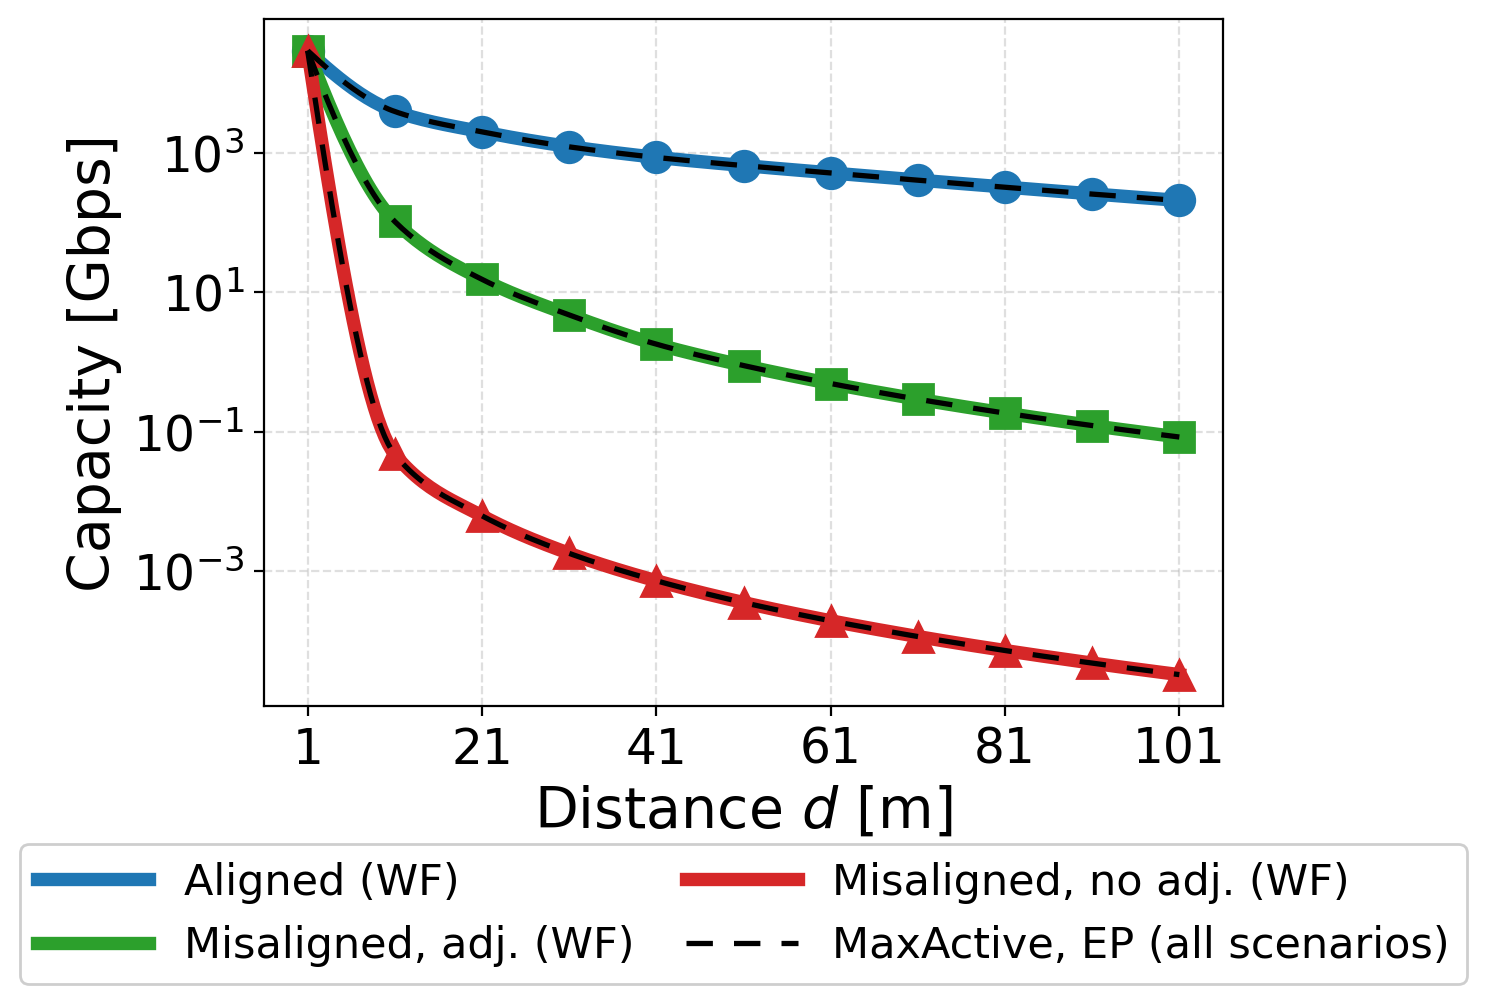
\includegraphics[width=\columnwidth]{maxactive_reference_single.png}}
\caption{MaxActive reference capacity versus distance for the aligned link and for
diagonal mobility with and without beamwidth adjustment, under WF (thick, solid) and EP
(thin, dashed) allocation. The three scenarios occupy disjoint decades of the logarithmic
axis, and WF and EP nearly coincide. Curves are PCHIP-smoothed, with markers at the
computed distances.}
\label{fig:maxactive}
\end{figure}

Fig.~\ref{fig:allmethods} overlays one representative of each regressor family, together
with the D3QN policy, on the MaxActive curves of the aligned and diagonal scenarios, and
Fig.~\ref{fig:mlmob} does the same for the elevation and real-trace scenarios. In the
elevation scenario without adjustment, the capacity stays high while the Rx is inside the
half-power beam and then drops to a side-lobe plateau once $\phi$ leaves the beam. With
adjustment, the beam widens and the capacity declines gradually instead. In the real
traces, the diagonal drift produces a sharp collapse that the measured accelerations
modulate with jitter, and because the trajectory begins at the reference initial distance
of $1$~m, the curve starts from a high capacity. In both figures, the kernel and
instance-based representatives follow the reference closely, the linear representatives
lag behind the reference, and the D3QN lies on the MaxActive curve throughout.

\begin{figure*}[!t]
\centerline{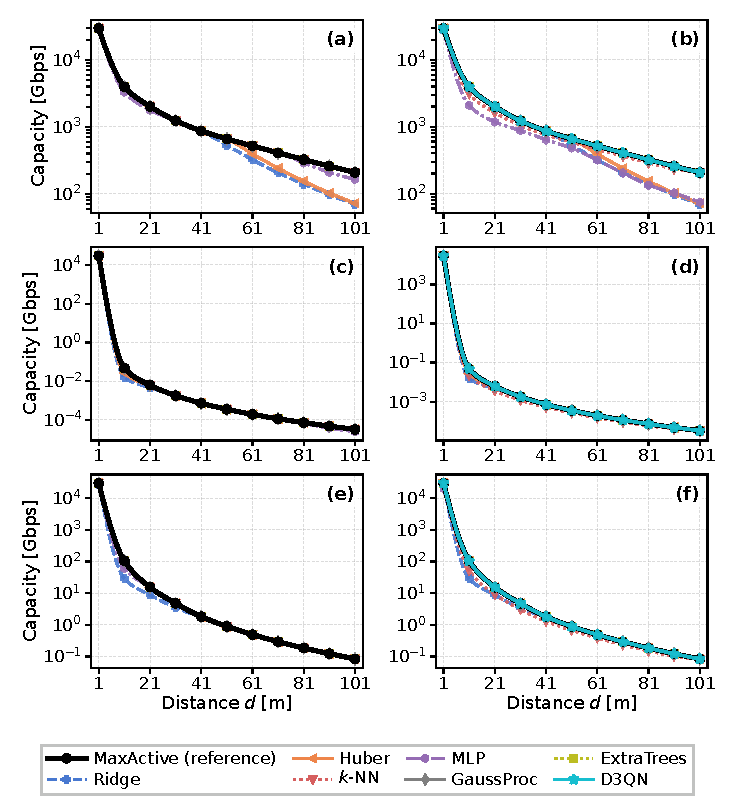
\includegraphics[width=4.9in]{fig_capacity_main.pdf}}
\caption{Learned models versus MaxActive in the aligned and diagonal scenarios.
Rows: (a), (b) aligned; (c), (d) misaligned diagonal mobility without beamwidth
adjustment; (e), (f) misaligned diagonal mobility with beamwidth adjustment. Columns: WF
target in (a), (c), (e) and EP target in (b), (d), (f); the D3QN, which uses EP, appears
in the EP column. One regressor per family is shown; all eighteen are compared in
Table~\ref{tab:cv}. Regressor curves are models fit on all $33$ samples, clipped at the
MaxActive ceiling \eqref{eq:clip} for display only (a deployed regressor has no access to
the ceiling), and PCHIP-smoothed with markers at the computed points.}
\label{fig:allmethods}
\end{figure*}

Table~\ref{tab:cv} gives the nested cross-validated metrics for the EP target, ranked by
RMSE. The WF target was cross-validated in the same way, and the two targets agree to
within $0.055$ RMSE for every one of the eighteen models and to within $0.021$ for all but
the single decision tree, as the near-equality of the WF and EP capacities in
Table~\ref{tab:maxactive} implies; only the EP column is therefore tabulated. The table
leads to three findings. First, the smooth nonparametric and kernel models perform best.
The Gaussian process leads by a wide margin ($R^2=0.99$, median relative error
$\approx1.9\%$), followed by ExtraTrees, SVR-RBF, MLP, and $k$-NN. The leading models assume
the smoothness that the physical capacity surface exhibits, so they interpolate MaxActive
closely and generalize across folds. Second, the regularized linear models are stable but
biased. Ridge, Lasso, ElasticNet, and BayesianRidge hold $R^2\approx0.97$ with small
variance, yet their $\approx45\%$ median relative error reveals a systematic offset,
because a model that is affine in the features cannot capture the curvature of a capacity
that decays over nine decades. Third, cross-validation exposes failures that a single
split hides. On a single $75/25$ split, Huber regression is second only to the Gaussian
process (RMSE $0.183$), but under CV the Huber model falls to $R^2=0.93\pm0.10$. Ordinary
least squares looks acceptable on the same split ($R^2=0.991$) but is far worse under CV
($R^2=-7.98\pm31$), dominated by unlucky folds. Huber regression and ordinary least
squares, together with the single decision tree and gradient boosting, are the failing
methods. On $33$ points a single split cannot be trusted, and the nested-CV
mean$\,\pm\,$std is the basis for the ranking.

\begin{table}[!t]
\caption{Nested Cross-Validated Accuracy and Physical-Ceiling Violations
(EP Target, Ranked Best to Worst)}
\label{tab:cv}
\setlength{\tabcolsep}{2pt}
\renewcommand{\arraystretch}{1.12}
\begin{tabular*}{\columnwidth}{@{\extracolsep{\fill}}l c c c c r@{}}
\hline
& \multicolumn{3}{c}{Nested-CV generalization} & \multicolumn{2}{c}{Ceiling violations}\\
\cline{2-4}\cline{5-6}
Model & RMSE$\,\pm\,$std & $R^2$ & Med.\ rel. & pts. & max\\
\hline
GaussProc           & $0.100\pm0.23$ & $0.991$  & $1.9\%$      & $19$       & $2.7\%$\\
ExtraTrees          & $0.237\pm0.18$ & $0.986$  & $12.1\%$     & $1$        & $3.7\%$\\
SVR-RBF             & $0.253\pm0.22$ & $0.982$  & $7.8\%$      & $18$       & $318\%$\\
MLP                 & $0.254\pm0.21$ & $0.980$  & $21.1\%$     & $20$       & $226\%$\\
BayesianRidge       & $0.331\pm0.14$ & $0.976$  & $42.5\%$     & $17$       & $322\%$\\
$k$-NN              & $0.338\pm0.29$ & $0.959$  & $9.0\%$      & $11$       & $111\%$\\
XGBoost             & $0.342\pm0.16$ & $0.970$  & $36.9\%$     & $14$       & $38\%$\\
KernelRidge         & $0.356\pm0.33$ & $0.962$  & $16.0\%$     & $17$       & $223\%$\\
Lasso/ENet/Ridge    & $0.36$--$0.37$ & $0.97$   & $45$--$49\%$ & $17$--$19$ & $232$--$261\%$\\
GradBoost           & $0.412\pm0.21$ & $0.957$  & $38.4\%$     & $16$       & $2993\%$\\
RF/Bag./AdaBoost    & $0.44$--$0.45$ & $0.96$   & $49$--$62\%$ & $9$--$11$  & $97$--$246\%$\\
Huber               & $0.504\pm0.37$ & $0.930$  & $48.4\%$     & $17$       & $1102\%$\\
DecisionTree        & $0.561\pm0.32$ & $0.931$  & $48.0\%$     & $3$        & $3698\%$\\
LinearReg           & $3.281\pm8.78$ & $-7.98$  & $55.8\%$     & $15$       & $405\%$\\
\hline
D3QN (policy)       & ---            & ---      & $\sim\!0\%$  & $0$        & $0\%$\\
\hline
\end{tabular*}

\vspace{3pt}
{\footnotesize\noindent RMSE and $R^2$: $\log_{10}$ target; Med.\ rel.: median relative
error in linear Gbps; all from raw, unclipped out-of-fold predictions. ``pts.'': number
of the $33$ points at which the prediction exceeds the reference; ``max'': largest such
excess, i.e., what \eqref{eq:clip} conceals. ENet $=$ ElasticNet, RF $=$ RandomForest,
Bag.\ $=$ Bagging. D3QN row: capacity of the selected channel set relative to
MaxActive-EP (not a regression metric).\par}
\end{table}

The last two columns of Table~\ref{tab:cv} quantify how far the raw predictions exceed
the reference ceiling. The excess is what the display clip \eqref{eq:clip} conceals and
is the error a deployed regressor would actually commit, since a deployed regressor has
no ceiling to clip against. Every regressor exceeds the reference at one or more points,
so the size of the violation is a first-class selection criterion. The piecewise-constant
single tree and plain gradient boosting overshoot by thousands of percent, because they
cannot extrapolate the wide dynamic range, and a link budget dimensioned on such a
prediction would be badly optimistic. GaussProc and ExtraTrees, by contrast, stay within a
few percent. The D3QN capacity did not exceed the MaxActive-EP reference at any of the
evaluated geometries, as expected for a policy that selects among the same SNR-ordered
prefixes.

Table~\ref{tab:perscen} breaks the out-of-fold median relative error down by scenario for
the strongest models. For four of the five models, at least one misaligned scenario is
harder than the aligned one; $k$-NN, for example, rises to $20.1\%$ in the worst-SNR
regime (misaligned, no adjustment). The Gaussian process is the exception and stays
within $2\%$ in all three scenarios. SVR-RBF and KernelRidge stay within about $7\%$
everywhere, whereas ExtraTrees degrades in both misaligned scenarios. Stability across
scenarios, and not merely a low aggregate error, is what qualifies a model as a robust
predictor.

\begin{table}[!t]
\caption{Per-Scenario Median Relative Error (EP Target, Nested-CV Out-of-Fold Predictions)}
\label{tab:perscen}
\setlength{\tabcolsep}{4pt}
\renewcommand{\arraystretch}{1.12}
\begin{tabular*}{\columnwidth}{@{\extracolsep{\fill}}l c c c@{}}
\hline
& & \multicolumn{2}{c}{Misaligned (diagonal)}\\
\cline{3-4}
Model & Aligned & No adjustment & With adjustment\\
\hline
GaussProc    & $2.0\%$ & $1.9\%$  & $0.8\%$\\
SVR-RBF      & $2.6\%$ & $5.3\%$  & $6.9\%$\\
KernelRidge  & $4.9\%$ & $6.0\%$  & $5.3\%$\\
$k$-NN       & $1.2\%$ & $20.1\%$ & $0.7\%$\\
ExtraTrees   & $2.7\%$ & $12.2\%$ & $24.6\%$\\
\hline
\end{tabular*}
\end{table}

On the elevation and real-trace scenarios of Fig.~\ref{fig:mlmob}, fitting on all $60$
samples, the strongest models reproduce the curves closely: XGBoost, GradBoost, and
GaussProc reach median relative errors of $0.07\%$, $0.7\%$, and $2.8\%$ over the
elevation and real scenarios, with Huber regression next at $4.4\%$. The mobility errors
come from an in-sample fit, which flatters models such as GradBoost that fail under
cross-validation; Table~\ref{tab:cv}, and not the in-sample fit, is therefore the basis
for the ranking.

\begin{figure*}[!t]
\centerline{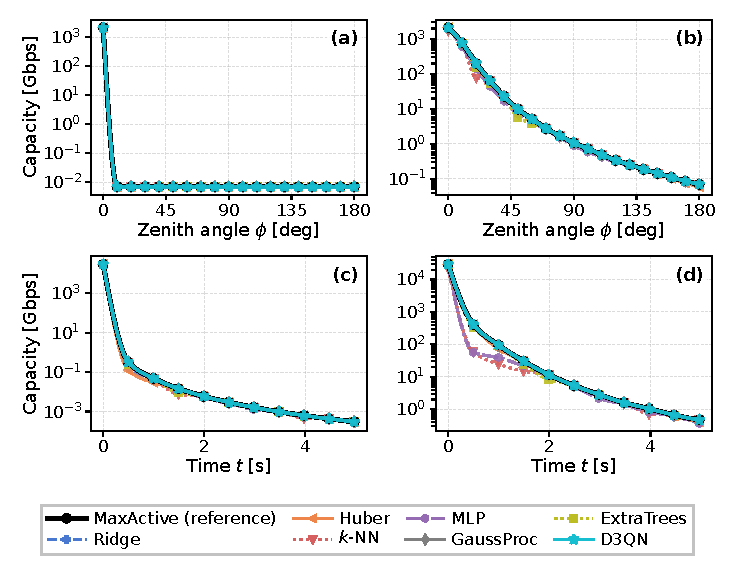
\includegraphics[width=4.9in]{fig_capacity_mobility.pdf}}
\caption{Learned models versus MaxActive on the two additional mobility patterns (EP
target): mobility over elevation (a) without and (b) with beamwidth adjustment, where
$\phi$ is the elevation (zenith) angle of the Rx seen from the Tx; and real windy-hover
traces (c) without and (d) with adjustment. Same model representatives as
Fig.~\ref{fig:allmethods}. WF panels are omitted because WF and EP coincide to within the
line width. Regressor curves are in-sample fits on the $60$ mobility samples, clipped at
the ceiling for display only, and PCHIP-smoothed. The D3QN (cyan) lies on the MaxActive
curve throughout.}
\label{fig:mlmob}
\end{figure*}

The D3QN, trained as a single-step contextual bandit at every trajectory point, reaches at
least $99.7\%$ of the MaxActive-EP capacity on all seven scenario variants. The mean
capacity ratio is $99.9\%$ for the aligned case and $100.0\%$ for each of the six
misaligned cases: diagonal, elevation, and real-trace mobility, each with and without
beamwidth adjustment. The worst single operating point over all $93$ evaluated geometries
($33$ in the main study plus $60$ mobility points) is $99.7\%$ of the reference, and no
point exceeds the reference. The selected channel counts are not always identical to
those of MaxActive; in the main study the counts differ by up to $30$ channels (e.g.,
$497$ versus $467$ at $81$~m in the aligned case). Near its maximum, the capacity is flat
in the number of active channels, so neighboring prefixes deliver almost the same
capacity. A policy operating at the same individual-channel granularity as MaxActive-EP
therefore returns a transmittable channel set of nearly reference capacity, under
elevation and real-trace mobility as well. The result is subject to the three
qualifications stated with the policy. The ratio is bounded by construction, because the
policy chooses among the same SNR-ordered prefixes; training uses the reference capacity
in the reward; and the reported decision is the better of the greedy action and the best
of the $1600$ actions evaluated during training \eqref{eq:aout}. The reported ratios
therefore characterize the complete training-plus-selection procedure, and how often the
greedy network output alone attains the ratios was not recorded.

The contrast between the regressors and the policy is the most transferable finding of
the study. A regressor predicts a number and can exceed the physical bound. The policy
predicts an allocation, and the capacity reported for the policy is the capacity that the
chosen allocation actually delivers, so the policy stays at or below the MaxActive-EP
reference ($99.7$--$100\%$) with no clip anywhere in the pipeline. Where an allocation
must be trusted without supervision, learning the decision is the safer target, subject
to the per-context training that the policy currently requires. The study also has
limitations that bound these claims. The datasets are small ($33$ and $60$ points) and
physically smooth, which favors smoothness-assuming models and restricts the validated
regime to interpolation within the trained envelope. The learned models imitate a
reference that is optimal only within its threshold-search family, so the models inherit
that scope rather than approximating a globally optimal allocation. The regressors
predict the capacity value rather than the channel set, so a system that needs the set
must use the policy, and the policy is trained per context rather than as a single
geometry-generalizing agent.


% ============================================================================
\section{CONVERGENCE AND COMPLEXITY}
\label{sec:complexity}
% ============================================================================
\subsection{ASYMPTOTIC COST}
MaxActive has a per-step cost of $O(Q\,|\mathcal{F}|)$ and must be re-run whenever the
geometry changes; the search needs no training but incurs its full cost at every time
step. The supervised models move the cost offline. The entire nested-CV benchmark of
$18$ models over both targets completes in about $30$~s on a CPU, dominated by the grid
searches, and fitting the $18$ deployable models on the full dataset takes $0.5$~s.
Afterwards, a prediction is a single forward, kernel, or neighbor evaluation.
Table~\ref{tab:complexity} summarizes the asymptotic training and prediction complexity
of representative families ($n$ samples, $d$ features, $T$ trees, $W$ network weights,
$n_{sv}$ support vectors), together with their measured cost and cross-validated
accuracy, and adds the MaxActive and D3QN references for context.

\subsection{MEASURED EXECUTION TIME}
\label{sec:runtime}
Asymptotic orders alone do not establish a practical benefit, so every stage was measured
on identical channel states, on a single core of an Intel Core i7-13620H, with the band
discretized into $|\mathcal{F}|=\PLNCH$ active channels per context. The measured columns
of Table~\ref{tab:complexity} average the eleven aligned contexts.

The reference costs \PLMASEL{} for the threshold sweep alone and \PLMASTEP{} for a
complete link update with power allocation iterated to convergence. On the three
geometries where both variants were timed, adding the beamwidth search raises the update
time from $72$~ms to \PLMASTEPBW{}, i.e., to $1.3\times$ the fixed-beam cost. The
regressor path, in comparison, costs $0.84$~ms to turn the channel state into the $13$
features and $21$--$43$~$\mu$s to evaluate a linear, kernel, or Gaussian-process model,
which amounts to \PLPREDUS{} end-to-end and an $88\times$ reduction in the per-update
decision cost. The model evaluation alone is $1800$--$3700\times$ faster than the search,
but feature extraction dominates the online path, so the end-to-end gain saturates near
two orders of magnitude, and feature extraction rather than inference is the target for
further optimization. The tree ensembles are the exception at the other end. Tree
ensembles need $3.0$--$12$~ms per prediction because hundreds of estimators must each be
traversed, which cuts their advantage to $6$--$20\times$ and makes the ensembles a poor
per-update choice at the present dataset size despite their accuracy. The D3QN gives the
fastest decision of all. The D3QN state is built from the SNR ranking that MaxActive
computes anyway ($0.55$~ms, shared by both methods), after which a forward pass and
$\arg\max$ take $0.05$~ms, three orders of magnitude below the search, and the policy
returns the channel set itself rather than a capacity estimate. The D3QN cost is paid
offline: $0.11$~s per context, or about $4$~s for the $33$ contexts of the main study.
Training one context thus costs more than one threshold sweep (\PLMASEL{}) and also needs
the reference capacity of the context. The per-context policy therefore saves computation
only when a trained context is revisited, and the online figure above applies to such
contexts.

\begin{table*}[!t]
\caption{Asymptotic and Measured Cost Versus Accuracy of Representative Models}
\label{tab:complexity}
\setlength{\tabcolsep}{3pt}
\renewcommand{\arraystretch}{1.15}
\begin{tabular*}{\textwidth}{@{\extracolsep{\fill}}l l l r r r c c@{}}
\hline
& \multicolumn{2}{c}{Asymptotic cost} & \multicolumn{3}{c}{Measured (single core, $n=33$)} &
  \multicolumn{2}{c}{Nested-CV accuracy (EP)}\\
\cline{2-3}\cline{4-6}\cline{7-8}
Model (family) & Training & Prediction & Train [ms] & Predict [ms] & Memory [KB] & $R^2$ & Med.\ rel.\ err.\\
\hline
Ridge / Lasso (linear)            & $O(nd^2)$              & $O(d)$                    & $0.7$        & $0.023$          & $1.2$          & $0.97$          & $45\%$\\
$k$-NN (instance-based)           & $O(1)$ (store)         & $O(nd)$                   & $0.5$        & $0.211$          & $7.6$          & $0.96$          & $9\%$\\
DecisionTree (tree)               & $O(nd\log n)$          & $O(\text{depth})$         & $0.4$        & $0.029$          & $5.3$          & $0.93$          & $48\%$\\
XGBoost / ExtraTrees (ensemble)   & $O(T\,nd\log n)$       & $O(T\,\text{depth})$      & $76$--$103$  & $0.32$--$11.7$   & $522$--$1362$  & $0.97$--$0.99$  & $12$--$37\%$\\
MLP (neural)                      & $O(\text{it}\cdot nW)$ & $O(W)$                    & $49$         & $0.031$          & $70$           & $0.98$          & $21\%$\\
SVR-RBF (kernel)                  & $O(n^2\!-\!n^3)$       & $O(n_{sv}d)$              & $0.8$        & $0.038$          & $4.6$          & $0.98$          & $8\%$\\
\textbf{GaussProc} (kernel/prob.) & $O(n^3)$, mem $O(n^2)$ & $O(n)$ mean               & $14$         & $\mathbf{0.043}$ & $\mathbf{17.9}$ & $\mathbf{0.99}$ & $\mathbf{1.9\%}$\\
\hline
MaxActive (reference)             & --- (online search)    & $O(Q|\mathcal{F}|)$ / step & ---         & $\mathbf{76.8}$  & ---            & reference       & ---\\
D3QN (policy)                     & $O(E\cdot A)$ / context & $O(\text{forward pass})$  & $115$/ctx.  & $0.05$           & $84$           & $\approx$ ref.  & $\sim\!0\%$\\
\hline
\multicolumn{8}{@{}p{\textwidth}@{}}{Prediction times are per operating point and exclude
the $0.84$~ms feature extraction shared by all regressors; the MaxActive row is the
threshold sweep alone, on the same channel states. Memory is the serialized model size;
the D3QN size corresponds to $21\,561$ parameters in single precision. For the D3QN, $E$ is the
number of training epochs and $A$ the number of actions evaluated per epoch.}\\
\end{tabular*}
\end{table*}

\subsection{MEMORY FOOTPRINT AND AIRBORNE DEPLOYMENT}
\label{sec:deploy}
For a UAV, memory and predictability matter as much as speed. The deployable models are
small: the regularized-linear models occupy $1.2$--$2.2$~KB, SVR-RBF $4.6$~KB, the
Gaussian process $17.9$~KB (its $33\times33$ kernel and training inputs), the MLP
$70$~KB, and the D3QN $21\,561$ parameters, i.e., $84$~KB in single precision. Models of
this size are compatible with the on-chip memory of microcontroller-class flight
companions, and all are far smaller than the LBLRTM tables that the reference search
itself must hold. Only the tree ensembles are heavy, with XGBoost at $522$~KB and
ExtraTrees at $1.4$~MB, which, together with their millisecond-scale inference, makes the
ensembles a poor fit here despite their accuracy. Three further properties favor
deployment. The inference cost is constant and independent of the data, a fixed number of
multiply-accumulates with no search, iteration, or early exit, so the decision has a hard
worst-case latency that a threshold sweep of state-dependent length cannot offer. All
training is offline, so the platform performs no gradient computation. Finally, the
arithmetic could be compressed further: an $8$-bit D3QN would occupy about $21$~KB (not
evaluated here), and the linear models reduce to a $13$-element dot product. On these
grounds, the Gaussian process is the better choice where accuracy dominates ($18$~KB,
$43$~$\mu$s), and the D3QN where the channel set is needed ($84$~KB, $0.05$~ms, subject
to per-context training). The tree ensembles are best reserved for offline or
ground-station use. The reported sizes and latencies indicate feasibility within the
memory and latency budgets of a flight companion. All timings, however, come from a
laptop-class CPU, so absolute latencies on an embedded airborne processor will be larger.
The ratio between search and learned model is expected to carry over approximately,
since both run on the same processor, but the ratio has not been measured on embedded
hardware, and a full airborne demonstration remains future work.

\subsection{CONVERGENCE}
For the supervised models, convergence is that of their standard solvers and is not a
limiting factor; the cost lies in the offline grid search. For the D3QN, the single-step
formulation removes bootstrapping variance and the credit-assignment horizon, which makes
training well conditioned. With the budget of $20$ epochs of $80$ actions, the returned
decision \eqref{eq:aout} reached $99.7$--$100\%$ of the reference capacity in all four
mobility patterns. Because \eqref{eq:aout} also considers the actions explored during
training, the budget is a measured sufficient setting for the complete procedure, not a
convergence result for the greedy network alone. Learning curves of the greedy action
were not recorded and are left to future work. The coupled power-allocation and MaxActive
loop inside the reference stops when the two channel sets agree and is capped at $30$
iterations; the iteration counts of the loop were not recorded.

\subsection{ACCURACY VERSUS COMPLEXITY}
The results reveal a clear accuracy-versus-complexity trade-off, which is the central
practical conclusion of the study. The most accurate model, the Gaussian process, has the
highest asymptotic training cost ($O(n^3)$ time, $O(n^2)$ memory, and a prediction that
requires the full training kernel). The next best models, SVR-RBF and kernel ridge
regression, are likewise kernel based at $O(n^2\!-\!n^3)$, and the cheapest models
($O(nd^2)$ training, $O(d)$ prediction) are systematically biased ($\approx45\%$ median
error). The accuracy ranking of Table~\ref{tab:cv} therefore roughly tracks the
asymptotic cost ranking of Table~\ref{tab:complexity}: the last few percent of accuracy
are bought at a super-linear price in the number of samples.

Two regimes invert the recommendation, however. At the present scale ($n\le60$), the
asymptotic penalty is invisible in wall-clock terms. The Gaussian process trains in
$14$~ms and predicts in $43$~$\mu$s, which is cheaper at inference than $k$-NN or any
ensemble, so the most accurate model can be chosen without a practical penalty, and the
Gaussian process is the model we recommend at the present scale. The time cost at the
present scale comes from the number of estimators rather than the asymptotic class,
which is why the tree ensembles are the slowest predictors in the table. As $n$ grows
toward the $10^4$--$10^6$ samples that denser simulation grids would provide, the cubic
training cost and quadratic memory of the kernel methods become prohibitive, while the
ensembles amortize their per-tree overhead, and the balance shifts to XGBoost and
ExtraTrees. A reasonable guideline is therefore to prefer kernel methods while the
dataset is small and tree ensembles once the dataset is large.


% ============================================================================
\section{CONCLUSION}
\label{sec:conc}
% ============================================================================
This paper studied spectrum allocation for THz UAV links, where molecular absorption,
absorption noise, and mobility-induced beam misalignment make the choice of active
channels and their powers decisive for capacity. Taking the MaxActive threshold search as
the reference solution, we investigated two machine-learning alternatives that work from
the same physical channel state: supervised regressors that predict the capacity the
search achieves, and a D3QN contextual-bandit policy that learns the channel selection
itself.

Three findings carry beyond the present system. First, the inductive bias that matters is
smoothness. The capacity surface is smooth and wide-ranging, so kernel and
Gaussian-process models track the reference closely, whereas piecewise-constant learners
cannot extrapolate the surface and overshoot the physical bound by orders of magnitude.
Second, on datasets of the present size, the evaluation protocol decides the ranking. A
single split reorders the models and hides overfitting, so nested cross-validation is a
requirement rather than a refinement. Third, learning the decision is safer than learning
its value. A policy that selects channels reports only capacities that a transmittable
allocation actually delivers, whereas a value regressor can predict a rate the link
cannot support.

In terms of cost, once trained, both learned branches lower the online decision cost by
about two orders of magnitude or more relative to the search, and both fit in the memory
of a small flight computer. For the regressors, feature extraction rather than inference
now limits the speed-up. At the present scale, the Gaussian process is the preferred
capacity predictor, and the D3QN is preferred where the channel set is needed. Only as
the dataset grows by orders of magnitude does the super-linear cost of kernel methods
favor tree ensembles. Three caveats bound the conclusions. First, the D3QN branch is
trained per operating context with the reference capacity in its reward, and the reported
decision also draws on the actions explored in training; the branch therefore covers a
pre-enumerated trajectory envelope rather than an arbitrary unseen geometry and pays off
only when trained contexts recur. Second, the regressors are validated as interpolators
within the trained envelope. Third, all timings come from a laptop-class CPU. Future work
will replace the per-context bandits with a single geometry-generalizing policy, evaluate
the greedy policy without the training-time fallback, predict the channel set rather than
only the capacity, validate on embedded hardware, and extend the dataset into the regime
where the complexity trade-off binds.

\section*{ACKNOWLEDGMENT}
In this work, AI tools are used for language editing purposes only, including correction
of grammatical errors, improvement of clarity, and enhancement of overall coherence. All
technical content, modelling choices, results, and conclusions are developed and verified
by the authors.

\bibliographystyle{IEEEtran}
\bibliography{References}

\end{document}
